\documentclass{article}
\usepackage[margin=0.8in]{geometry}
\usepackage{amsmath}
\usepackage{ctex}
\usepackage{siunitx}
\usepackage{multirow}
\usepackage{bigstrut}
\usepackage{graphicx}
\usepackage{hyperref} 
\usepackage{mathbbol}

\title{干涉法测微小量数据处理}
\author{姓名:宋建宏\,\, 学号:PB21020677\,\, 班级:203院22级5班\\ 日期:2023年5月16日}
\date{}

\begin{document}
\maketitle

\section*{实验目的}
掌握组装、调整衍射光路的方法。使用不同结构衍射屏实现夫琅禾费衍射,观察实验现象,研究不同结构衍
射屏的衍射光强分布特征。结合理论计算衍射屏的结构参数,(单缝的缝宽,双缝中心间距)。

\section*{实验原理}
本实验讨论夫琅禾费衍射。
\subsection*{单孔衍射}
光通过小孔发生衍射,在接收屏上呈现出一个中央亮斑和
环绕中央亮斑的环状衍射图样。大约有 84\%的光强集中于中央亮斑,这个亮斑
被称为艾里斑。
\subsection*{单缝衍射}
利用能发出平行光的波源, 通过单缝后在一个接收屏上可以收到衍射图样。 由惠更斯一菲涅尔原理可知, 单缝上的每个点都可以看做是新的波源。这些波 源发出的子波在接收屏上叠加, 由理论计算得, 其光强分布表现为:
$$
I_{\varphi}=I_0\left(\frac{\sin u}{u}\right)^2 \text {, 其中 } u=\pi a \frac{\sin \varphi}{\lambda}
$$
式中 $a$ 为单缝的宽度, $I_0$ 为入射光光强, $\varphi$ 为衍射光与光轴的夹角, 即衍射 角。当衍射角 $\varphi$ 固定时, 观察点的光强值与波长 $\lambda$ 和单缝缝宽 $a$ 有关。
当 $u=0$ 即 $\varphi=0$ 时, $I_\varphi$ 取得最大值, 即 $I_0$, 此时对应的衍射亮斑在所有条纹中 最亮,被称为中央主极大。而
$$
a \sin \varphi=k \lambda \text { 时, } k=0, \pm 1, \pm 2, \pm 3 \ldots
$$
时, 有 $u=k \pi$, 即 $\sin u=0$, 表现为暗纹。此时衍射角对应的位置为暗纹的中 心。在本实验中, 衍射角 $\varphi$ 很小, 可以认为 $\sin \varphi=\varphi$, 于是有
$$
\varphi=\frac{k \lambda}{a}
$$
即
$$
\varphi=\frac{k_x}{L}=\frac{k \lambda}{a}
$$
\subsection*{双缝衍射}
双缝元件狭缝的宽度为 $a$, 中间不透光部分宽度为 $\mathrm{b}$, 则双缝中心间 距 $\mathrm{d}=a+\mathrm{b}$. 因此, 屏上 $P_{\varphi}$ 处的光强分布为
$$
I_{\varphi}=4 I_0\left(\frac{\sin u}{u}\right)^2 \cos ^2 v
$$
其中 $u=\pi a \frac{\sin \varphi}{\lambda}, \mathrm{v}=\pi d \frac{\sin \varphi}{\lambda}$;
上式表明:双缝衍射的光强由两个因素共同决定。其中 $\mathrm{u}$ 是单缝衍射带来的 决定项, 而 $\mathrm{v}$ 表示两个缝产生的两束光的相位差带来的影响结果。因此双缝夫
琅禾费衍射的光强由两个因素乘积共同作用而成。
因此, 当两个因子有一个值为 0 时, 接收屏上接收到的图像为暗纹。

对 $\mathrm{u}$ 而言, 使得 $\frac{\sin u}{u}$ 为 0 的条件是: $u=\pi a \frac{\sin \varphi}{\lambda}=k \pi$, 即
$$
a \sin \varphi=k \lambda, k \in \mathbb{Z} \text { 且 } k \neq 0
$$

对 $\mathrm{v}$ 而言, 使得 $\cos ^2 \mathrm{v}=0$ 的条件是: $v=\pi d \frac{\sin \varphi}{\lambda}= \pm\left(m-\frac{1}{2}\right) \pi$, 即
$$
d \sin \varphi= \pm\left(m-\frac{1}{2}\right) \lambda, m \in N^*
$$
同样, 出现衍射极大值的条件是: $v=\pi d \frac{\sin \varphi}{\lambda}=n \pi$, 即
$$
d \sin \varphi=\mathrm{n} \lambda, \mathrm{n} \in \mathbb{Z}
$$
但是, 当 $d \sin \varphi=\mathrm{n} \lambda, \mathrm{n} \in \mathbb{Z}$ 确定的最大值与 $a \sin \varphi=k \lambda, k \in \mathbb{Z}$ 且 $k \neq 0$ 确定的最小值 重合时, 第 $\mathrm{n}$ 级干涉条纹不会出现,这种现象称为缺级。第 $\mathrm{n}$ 级缺级的条件是:
$$
\frac{n}{k}=\frac{d}{a}
$$
根据以上推导可得:当狭缝宽度较小时, 尤其是小于光的波长时, 观察到的 衍射条纹, 从中央向两端的亮度基本不衰减; 同时, 条纹之间的间距与屏与双 缝的距离成正比,与双缝间距成反比。

\section*{实验仪器}
光学导轨及附件,He-Ne 激光器(632.8 nm)及电源,衰减片,衍射元件(单缝,双缝,圆
孔等),CCD,一维平移台,显示屏,支架,弹簧,细金属丝等。 
\section*{测量记录}
见原始数据

\section*{数据处理}
光路中L的长度为\(
    L=82.00-40.00-2.00=\SI{40.00}{cm}=\SI{0.4}{m}\)
\subsection*{单缝衍射}
    使用Origin进行线性拟合如图
    \begin{figure*}[htbp]
        \centering
        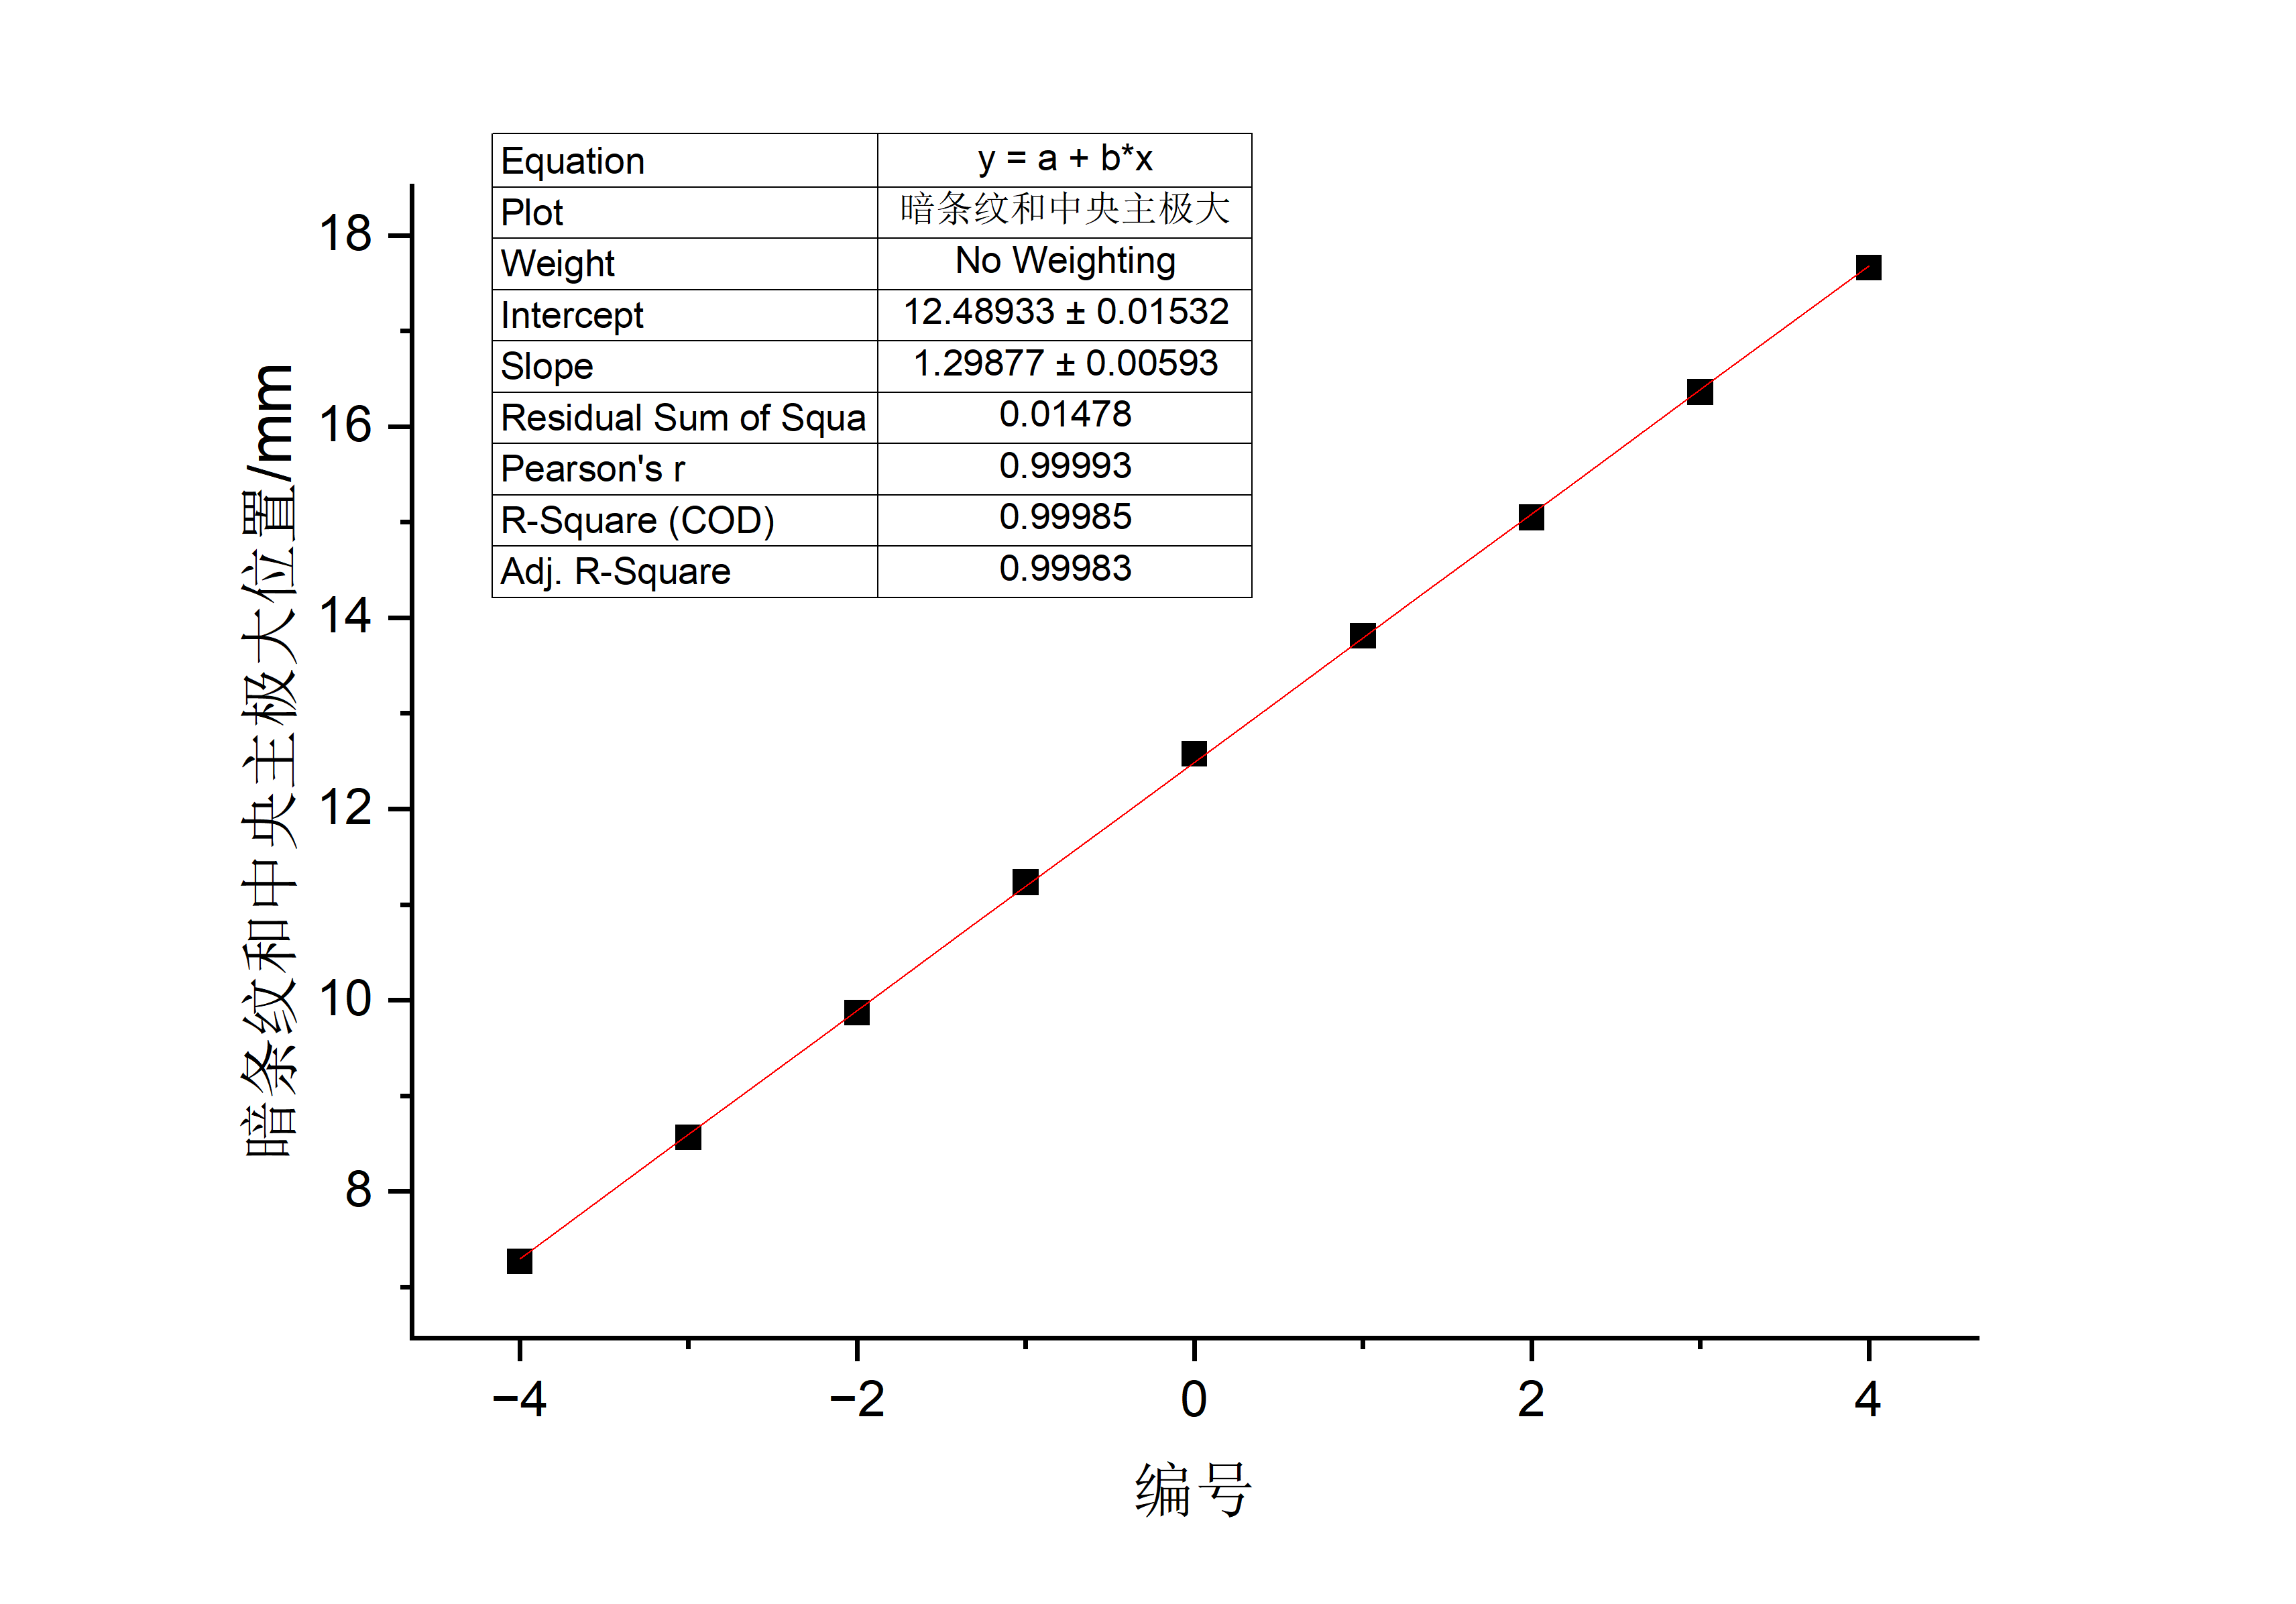
\includegraphics[scale=0.35]{graph2.png}
    \end{figure*}

    得图象斜率绝对值约为1.299,即\[\left|\frac{k}{x_k-x_0}\right|=\frac{1}{1.299\times 10^{-3}}m^{-1}=796.96m^{-1}\]
    得单缝缝宽
    \[a=\lambda L\left|\frac{k}{x_k-x_0}\right|=632.8\times10^{-9}\times0.4\times 796.96=201.7\mu m\]

\subsection*{双缝衍射}
线性拟合如图
    \begin{figure*}[htbp]
        \centering
        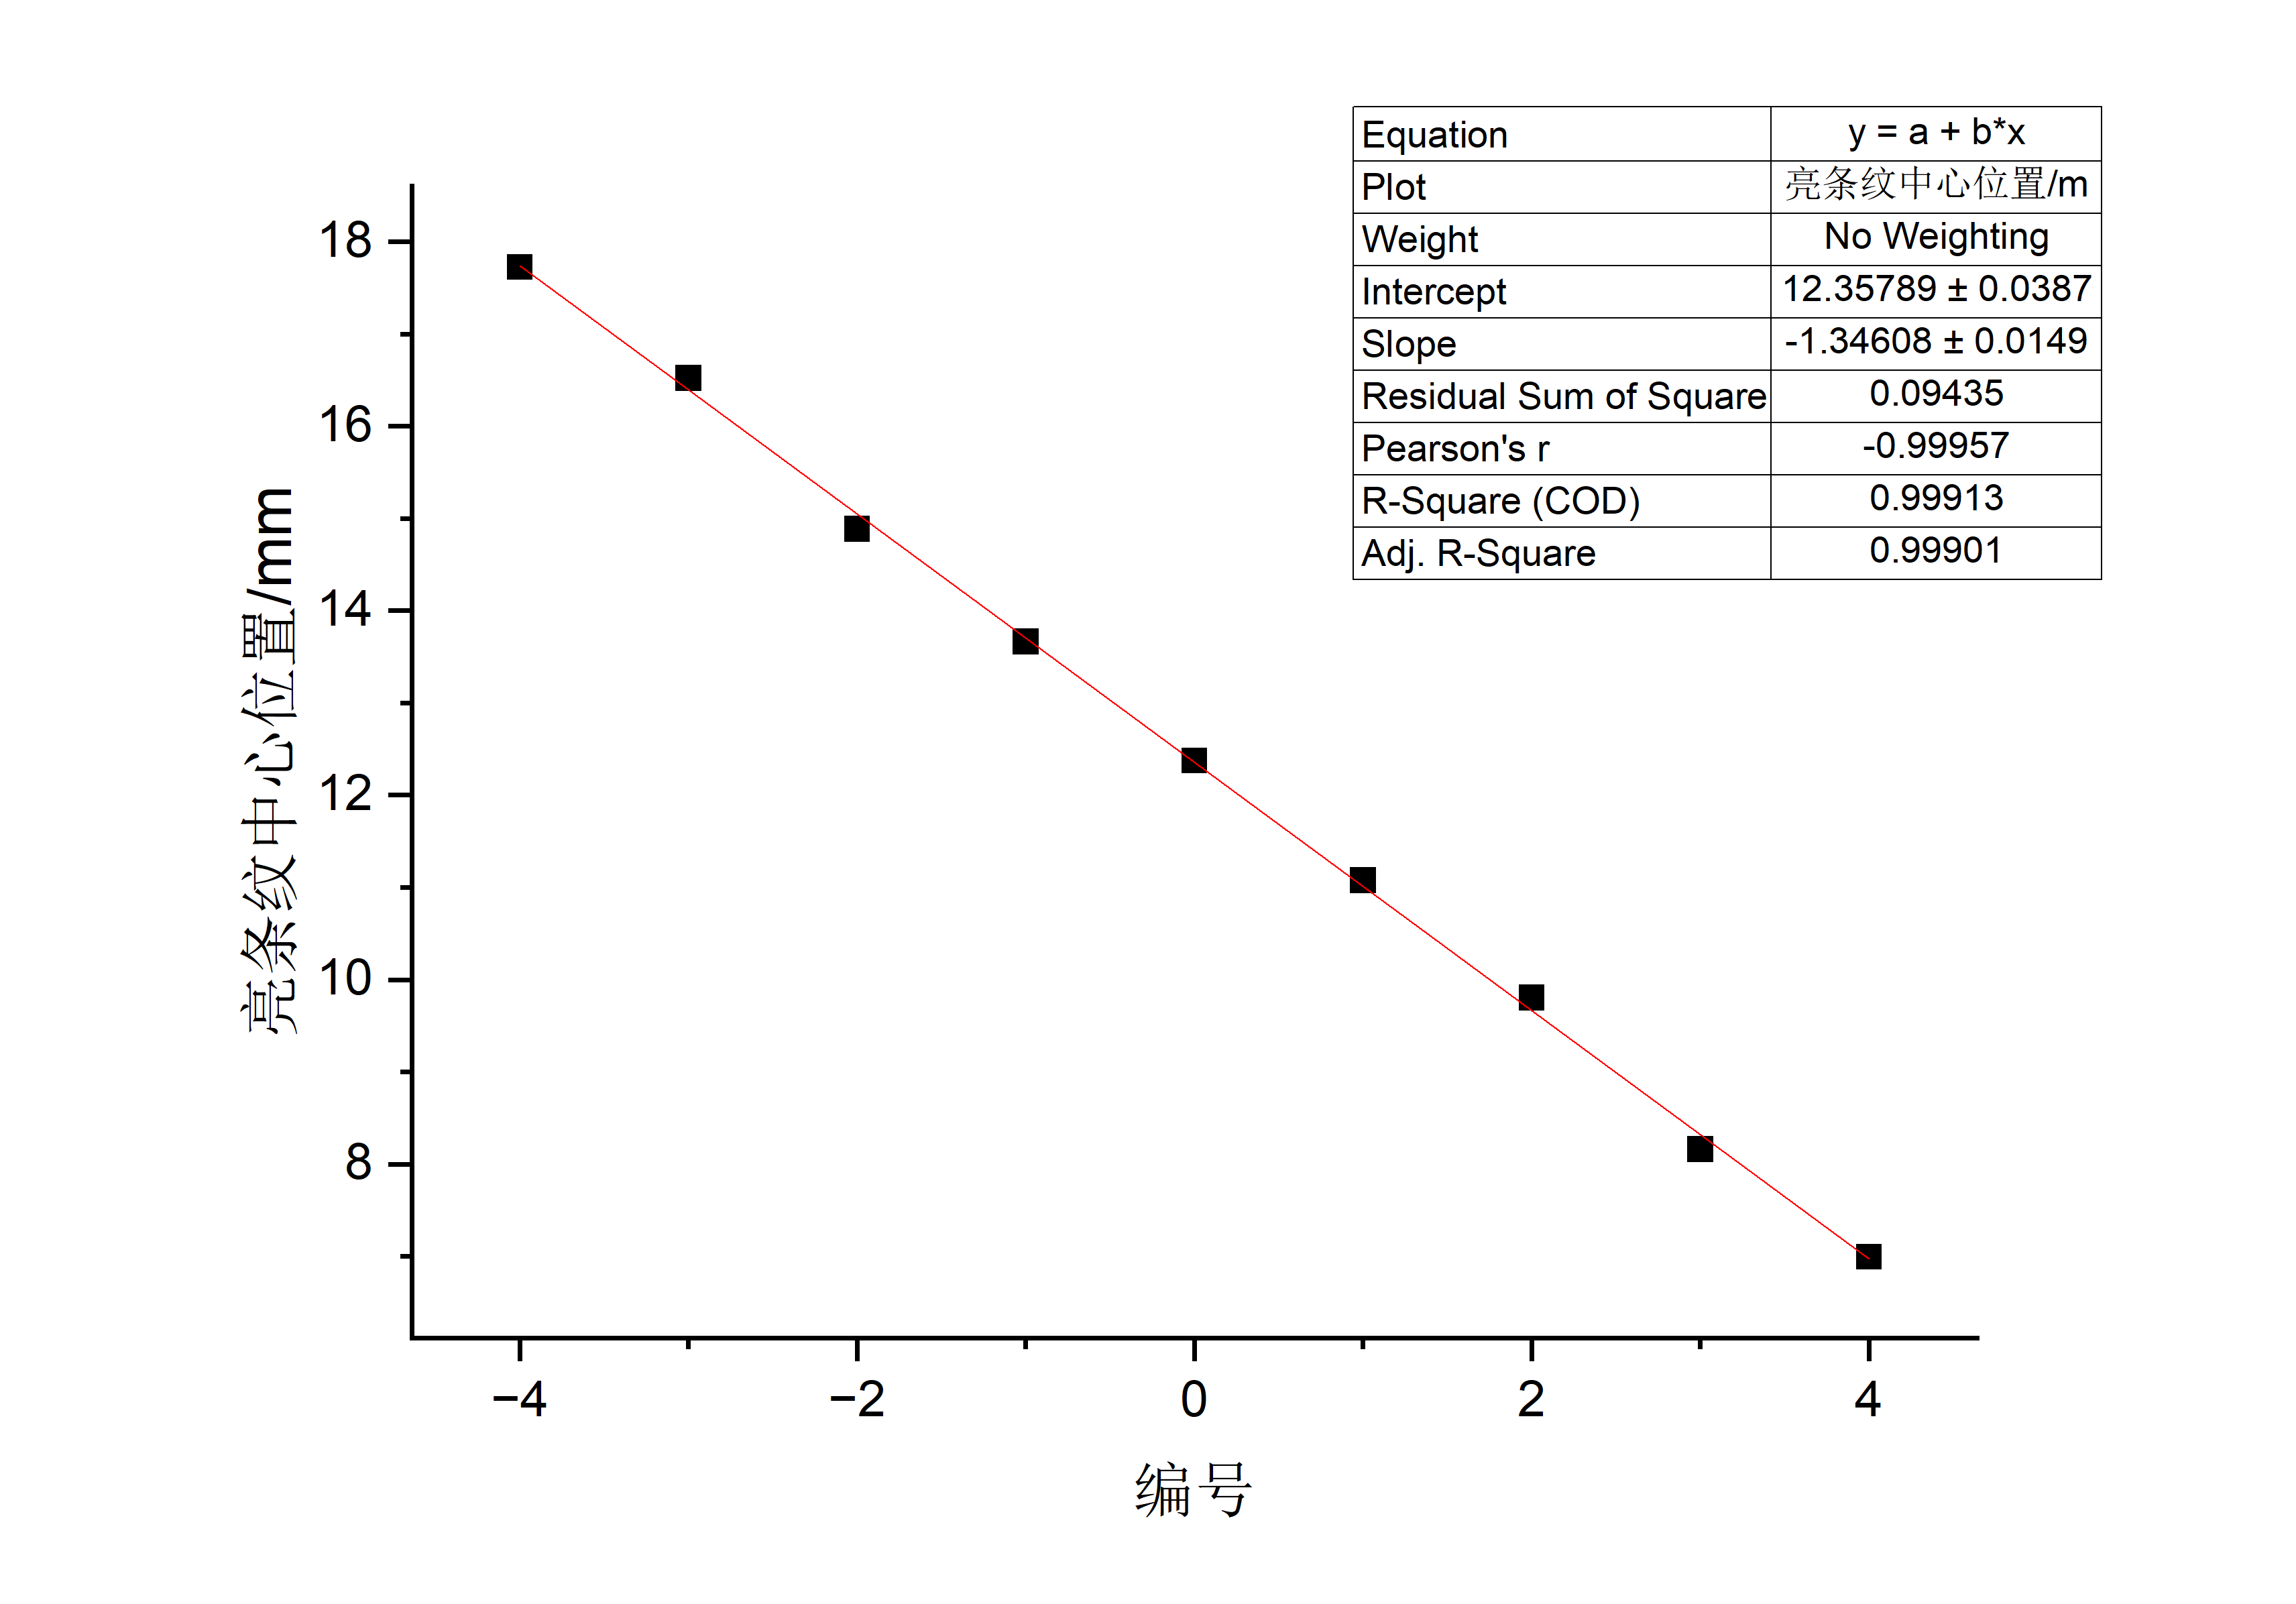
\includegraphics[scale=0.35]{graph0.png}
    \end{figure*}

    得图象斜率绝对值约为1.346,即\[\left|\frac{k}{x_k-x_0}\right|=\frac{1}{1.346\times 10^{-3}}m^{-1}=742.94m^{-1}\]
    则双缝间距为\[d=\lambda L\left|\frac{k}{x_k-x_0}\right|=632.8\times10^{-9}\times0.4\times 742.94=188.1\mu m\]

\section*{误差分析}


单缝的标定宽度为$\SI{200}{\mu m}$,相对误差为
\[\delta =\left|\frac{201.7-200}{200}\right|\times 100\%=0.85\%\]

双缝的标定间距为$\SI{190}{\mu m}$,相对误差为
\[\delta =\left|\frac{188.1-190}{190}\right|\times 100\%=1\%\]

总体来看相对误差较小。
\subsection*{误差来源}
\begin{enumerate}
    \item CCD镜头的凸出距离无法精确测量,导致L不够精确。
    \item 衍射图象边界较模糊,较难精准测量衍射光斑位置。
    \item 调节ccd镜头的齿轮具有回程差,测量时只能单向转动,无法精确测量光斑位置。
    \item 光路中的衍射元件难以调整至与光线垂直。
\end{enumerate}






\section*{思考题}
\begin{enumerate}
    \item 当光通过一个小孔时,在后面的光屏上会得到什么样的图案?
    
    若小孔较大,则仅仅出现一个光斑;当小孔较小时,出现一个夫
琅禾费小孔衍射图案。如果是多颜色叠加的光,则其衍射条纹将有不同色光分布。

    \item 白光照射到狭缝上,衍射条纹有什么特点?
    
    中间形成白色亮条纹,两边分布不同颜色的彩条纹。

    \item LED 射灯照到手机屏幕时可观察到下图中的现象,解释其原因。
    
    光在手机屏幕透明层里多次折射和衍射,可以形成这种状态。
\end{enumerate}


\end{document}